%-- coding:UTF-8 --

\documentclass{article}

\usepackage[english]{babel}
\usepackage[UTF8]{ctex}
\usepackage{listings}
\usepackage{xcolor}
\usepackage{float}

\lstset{
  language=bash,
  basicstyle=\small\ttfamily,
  keywordstyle=\color{blue}\bfseries,
  commentstyle=\color{green},
  stringstyle=\color{red},
  showstringspaces=false,
  showtabs=false,
  numbers=left,
  stepnumber=1,
  numbersep=10pt,
  tabsize=4,
  breaklines=true,
  frame=single,
}

\usepackage[letterpaper,top=2cm,bottom=2cm,left=3cm,right=3cm,marginparwidth=1.75cm]{geometry}

\usepackage{amsmath}
\usepackage{graphicx}
\usepackage[colorlinks=true, linkcolor=black, filecolor=black, urlcolor=black]{hyperref}


\title{实验报告1:版本控制(Git)}
\author{方欣 23020007021}
\date{}

\begin{document}
\maketitle

\tableofcontents
\thispagestyle{empty}			
\addtocontents{toc}{\protect\thispagestyle{empty}}

\newpage
\section{github链接}
\href{https://github.com/nixgnaf/SDT_report.github.io}{github 链接:https://github.com/nixgnaf/SDT_report.github.io}

\section{实验目的}
Git 是一个开源的版本控制系统,主要用于源代码管理。它能够帮助开发者跟踪文件的更改历史,协调多人合作开发,并处理分支和合并等任务。在 Git 中,文件的状态可以分为三种:已修改(modified)、已暂存(staged)和已提交(committed)。这使得Git项目拥有三个主要阶段:工作区、暂存区和Git目录。
\begin{itemize}
    \item 已修改表示当文件在工作区被修改但还未保存到数据库中时;
    \item 已暂存表示这些更改被标记为将要包含在下一次提交中;
    \item 已提交表示文件的更改被安全地保存到本地仓库的版本历史中;
\end{itemize}
Git 的常规操作流程包括:首先使用 \texttt{git clone} 克隆远程仓库到本地,接着在本地进行代码修改,通过 \texttt{git add} 将更改添加到暂存区,使用 \texttt{git commit} 提交更改到本地仓库。如果需要与远程仓库同步,则使用 \texttt{git pull} 拉取远程更改,解决任何可能的冲突,然后使用 \texttt{git push} 将本地提交推送到远程仓库。

本实验旨在初步掌握常见Git命令的基本用法,熟悉如何初始化仓库、管理文件、分支操作以及与远程仓库的交互。

\section{实验环境}
Git Bash:提供Unix风格的命令行工具。版本:Git-2.46.0-64-bit

操作系统:Windows 11

\section{实验内容}

\subsection{git clone}

\lstset{language=bash}
\begin{lstlisting}
git clone https://github.com/missing-semester-cn/missing-semester-cn.github.io
\end{lstlisting}

\noindent git clone:用于克隆远程仓库的git 命令,将远程仓库的内容复制到本地,并创建一个与远程仓库同步的本地仓库副本。

\noindent https://github.com/missing-semester-cn/missing-semester-cn.github.io:指向一个托管在 GitHub 上的 Git 仓库的位置.

\begin{figure}[h]
    \centering
    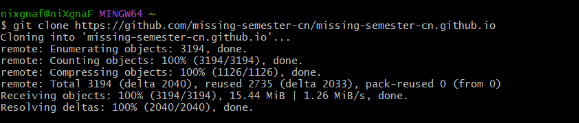
\includegraphics[width=1\linewidth]{picture/gitclone.png}
\end{figure}

\subsection{git remote add origin}
\lstset{language=bash}
\begin{lstlisting}
git remote add origin https://github.com/missing-semester-cn/missing-semester-cn.github.io
\end{lstlisting}

\noindent 这个命令将指定的远程仓库地址与本地仓库关联,使得可以进行远程操作,如推送和拉取代码.

\noindent git remote: 这是 Git 命令的一个子命令,用于管理远程仓库。

\noindent add: 这是 git remote 子命令中的一个操作,表示添加一个新的远程仓库。
在默认情况下,Git 使用 origin 作为远程仓库的默认名称。

\begin{figure}[h]
    \centering
    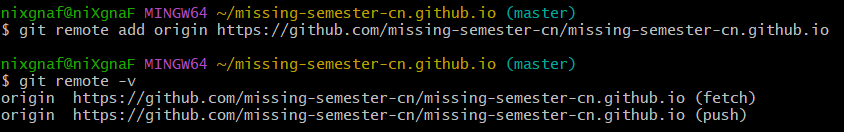
\includegraphics[width=1\linewidth]{picture/remoteadd.png}
\end{figure}

\subsection{git push origin}
\lstset{language=bash}
\begin{lstlisting}
git push origin master
\end{lstlisting}

\noindent git push :将本地仓库的更改推送到远程仓库

\noindent master: 这是本地分支的名称
\begin{figure}[h]
    \centering
    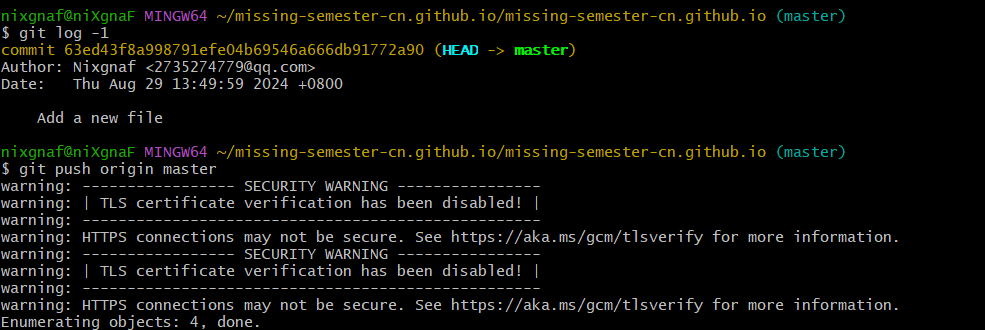
\includegraphics[width=1\linewidth]{picture/gitpush.png}
\end{figure}

\subsection{git log --all --graph –decorate}
\lstset{language=bash}
\begin{lstlisting}
git log --all --graph –decorate
\end{lstlisting}

\noindent git log: Git 用于查看提交历史的基本命令

\noindent --all: 显示所有分支的提交历史,确保看到仓库中的所有提交,不论它们属于哪个分支

\noindent --graph: 以图形化的方式显示提交历史。这个选项会在日志的左侧添加一个 ASCII 图形,用于可视化分支和合并的历史结构

\noindent 显示分支、标签和其他引用的名称。这个选项会在每个提交记录旁边显示当前分支和标签的位置,例如图中: (HEAD -> master, origin/master, origin/HEAD)
\begin{figure}[h]
    \centering
    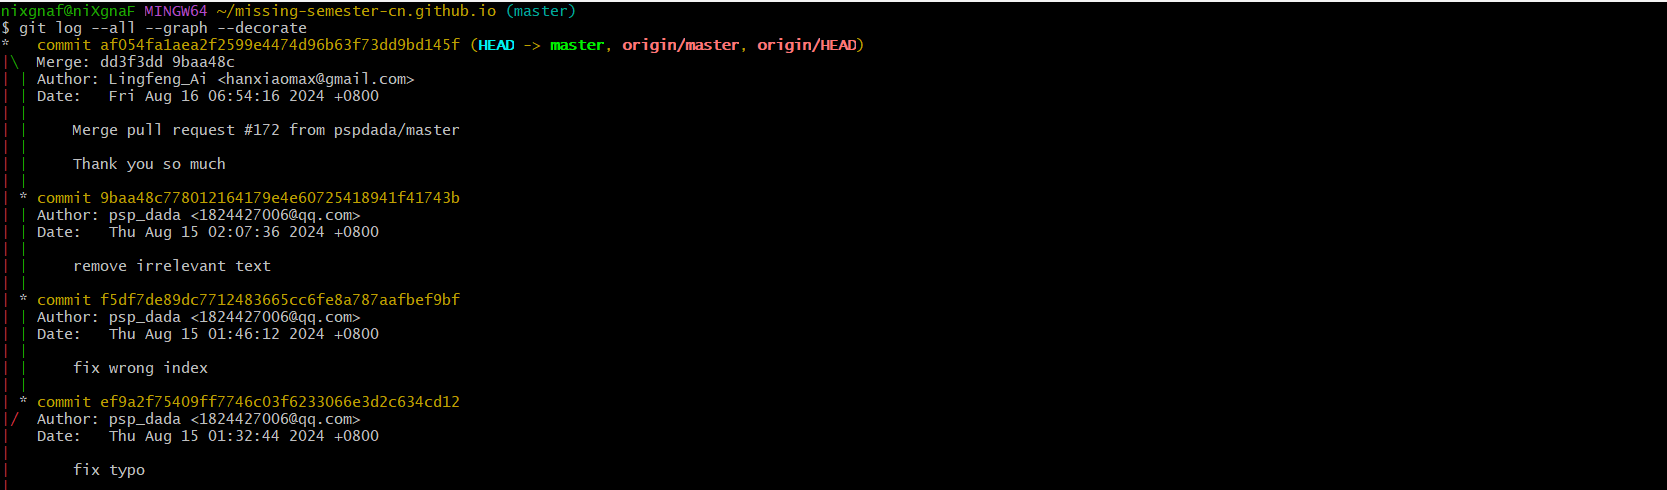
\includegraphics[width=1\linewidth]{picture/getlogall.png}
\end{figure}

\subsection{git log -p -n 1}
\lstset{language=bash}
\begin{lstlisting}
git log -p -n 1 README.md
\end{lstlisting}

\noindent -p:显示提交的详细变更内容(差异),即显示每个提交对 README.md 文件所做的具体修改。

\noindent -n 1:限制输出显示的提交数量,表示只显示最近的一次提交。

\begin{figure}[h]
    \centering
    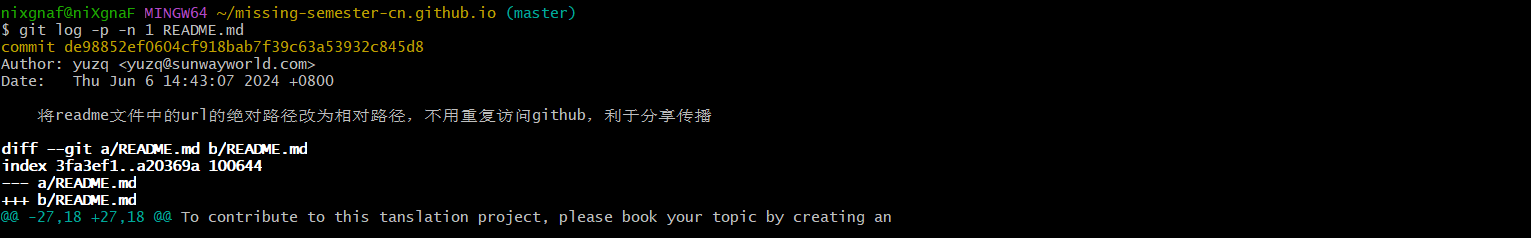
\includegraphics[width=1\linewidth]{picture/gitlog1.png}
\end{figure}

\subsection{git show a88b4eac}
\lstset{language=bash}
\begin{lstlisting}
git show a88b4eac
\end{lstlisting}

\noindent git show: 默认情况下,这个命令显示提交 a88b4eac 的详细信息,包括提交哈希、作者、日期、提交消息,以及该提交所做的所有更改(文件差异)。

\begin{figure}[h]
    \centering
    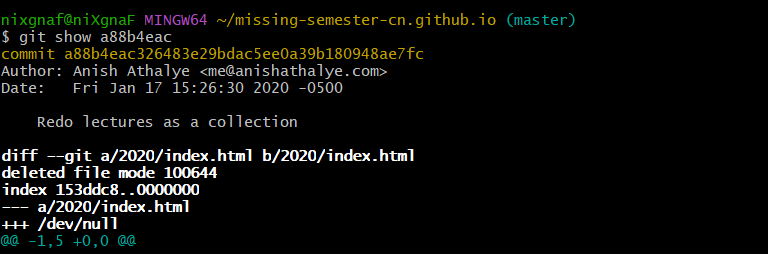
\includegraphics[width=1\linewidth]{picture/gitshow4.png}
\end{figure}

\subsection{git show --pretty=format:"\%s" a88b4eac | head -1}
\lstset{language=bash}
\begin{lstlisting}
git show --pretty=format:"%s" a88b4eac | head -1
\end{lstlisting}

\noindent git show --pretty=format:"\%s": 这个命令用于自定义格式化输出。--pretty=format:"\%s" 选项只会显示提交的消息(即提交说明)。

\noindent a88b4eac: 是提交的哈希值。

\noindent head -1: 只显示第一行。
\begin{figure}[h]
    \centering
    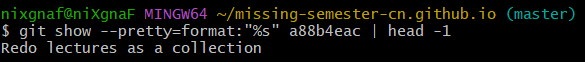
\includegraphics[width=1\linewidth]{picture/gitlogpretty.png}
\end{figure}

\subsection{git log --pretty=format:"\%s" a88b4eac -1}
\lstset{language=bash}
\begin{lstlisting}
git log --pretty=format:"%s" a88b4eac -1
\end{lstlisting}

\noindent --pretty=format:"\%s": 自定义输出格式。%s 代表提交消息的主题行(即提交说明的第一行)。

\noindent -1: 限制输出到最新的1个提交。
\begin{figure}[h]
    \centering
    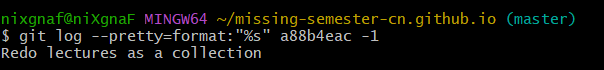
\includegraphics[width=1\linewidth]{picture/gitshowpretty.png}
\end{figure}

\subsection{git add .}
\lstset{language=bash}
\begin{lstlisting}
git add .
\end{lstlisting}

\noindent 将当前目录下的所有更改(包括新文件和修改的文件)添加到暂存区,以便进行提交。. 代表当前目录。

\begin{figure}[h]
    \centering
    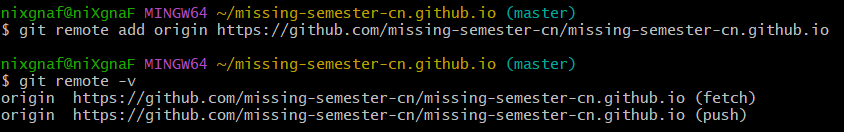
\includegraphics[width=1\linewidth]{picture/remoteaddd.png}
\end{figure}

\subsection{git commit -m "add password123 to file"}
\lstset{language=bash}
\begin{lstlisting}
git commit -m "add password123 to file"
\end{lstlisting}

\noindent Git commit: 于将暂存区的更改记录到本地版本库中,生成一个新的提交

\noindent -m: 用于指定提交消息。可在命令行中直接提供提交消息

\noindent "add password123 to file": 这是提交消息,描述这次提交所做的更改。消息应该简明扼要地说明提交的内容和目的
\begin{figure}[h]
    \centering
    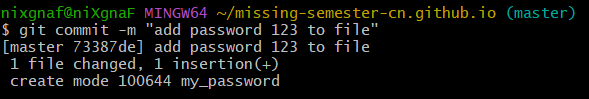
\includegraphics[width=1\linewidth]{picture/gitcommit.png}
\end{figure}

\subsection{git status}
\begin{lstlisting}
git commit -m "add password123 to file"
\end{lstlisting}

\noindent 用于查看当前工作目录和暂存区的状态。它提供了关于当前分支的状态、哪些文件被修改或尚未提交、以及其他有关版本控制的信息。
\begin{figure}[h]
    \centering
    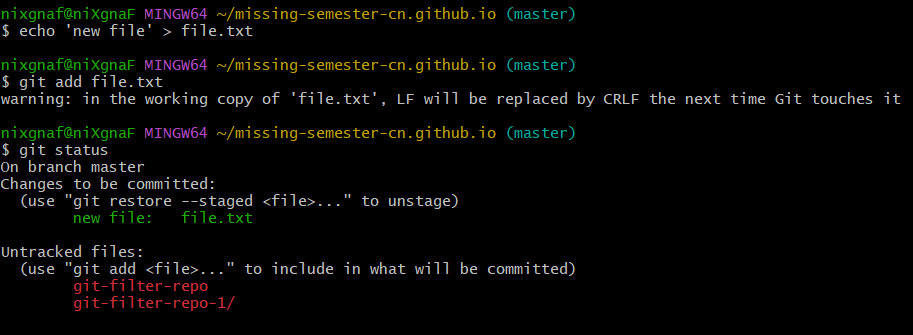
\includegraphics[width=1\linewidth]{picture/gitstatus.png}
\end{figure}


\subsection{git config --global core.excludesfile ~/.gitignore}
\begin{lstlisting}
git config --global core.excludesfile ~/.gitignore
\end{lstlisting}

\noindent 这条命令告诉Git在用户主目录下使用.gitignore文件作为全局忽略文件。
\begin{figure}[h]
    \centering
    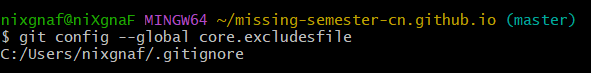
\includegraphics[width=1\linewidth]{picture/gitconfig.png}
\end{figure}

\subsection{git stash pop}
\begin{lstlisting}
git stash pop
\end{lstlisting}

\noindent git stash pop 命令用于将之前存储在 Git 暂存区中的更改(即 stash 中的内容)恢复到工作目录,并从 stash 中移除相应的记录。

\noindent 当你暂时存储了当前工作进度(使用 git stash),然后在完成其他任务后需要恢复这些进度时,可以使用 git stash pop。
\begin{figure}[h]
    \centering
    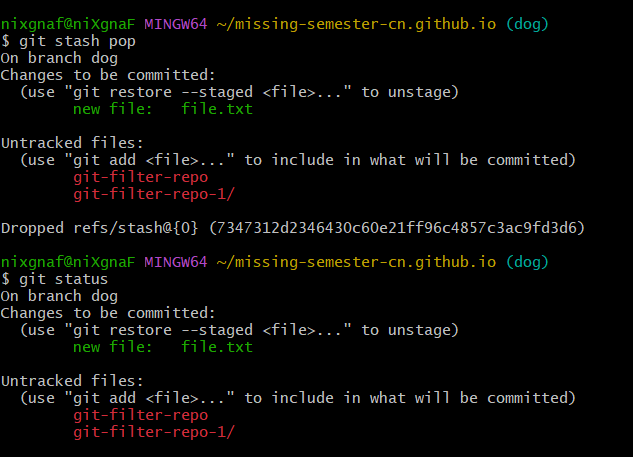
\includegraphics[width=1\linewidth]{picture/gitpop1.png}
\end{figure}

\noindent  
从main分支切换到dog分支,再将存储恢复,然后提交,这时,我们刚才新建的file.txt,变成了dog分支下的一次新提交。
\begin{figure}[h]
    \centering
    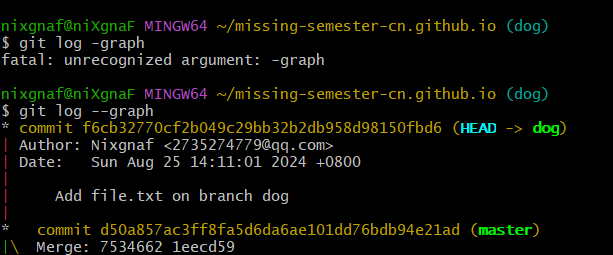
\includegraphics[width=1\linewidth]{picture/gitpop2.png}
\end{figure}

\subsection{[alias] graph = log --all --graph --decorate –oneline}
\begin{lstlisting}
[alias]graph = log --all --graph --decorate –oneline
\end{lstlisting}

\noindent 在 Git 的配置文件 ~/.gitconfig 中, [alias] 部分用于定义 Git 命令的别名。

\noindent 通过设置这个别名,可以使用 git graph 代替更长的命令 git log --all --graph --decorate --oneline。
\begin{figure}[h]
    \centering
    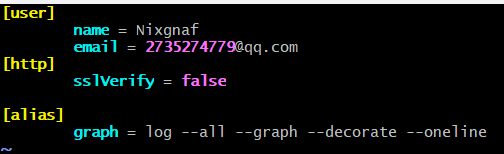
\includegraphics[width=1\linewidth]{picture/alias.png}
\end{figure}

\newpage
\subsection{git filter-branch}
\begin{lstlisting}
git filter-branch --force --index-filter\
 'git rm --cached --ignore-unmatch ./my_password' \
 --prune-empty --tag-name-filter cat -- --all

\end{lstlisting}

\noindent 这个命令的目的是从所有 Git 历史记录中的每个提交中删除文件 ./my\_password,并清理那些因为文件被删除而变得空的提交。

\noindent git filter-branch: 主命令,用于重写 Git 历史记录。允许你历史记录进行各种修改,例如删除文件、替换文件内容、修改提交信息等。

\noindent (使用git filter-repo代替实现功能)

\newpage
\subsection{git filter-repo –path my \_password –invert-paths}
\begin{lstlisting}
git filter-repo –path my_password –invert-paths
\end{lstlisting}

\noindent git-filter-repo 会重写仓库的历史记录,这可能包括删除某些文件、提交或者其他信息。

\noindent --path path/to/file 指定你要删除的文件路径。

\noindent --invert-paths 指定删除指定路径以外的所有内容。
\begin{figure}[h]
    \centering
    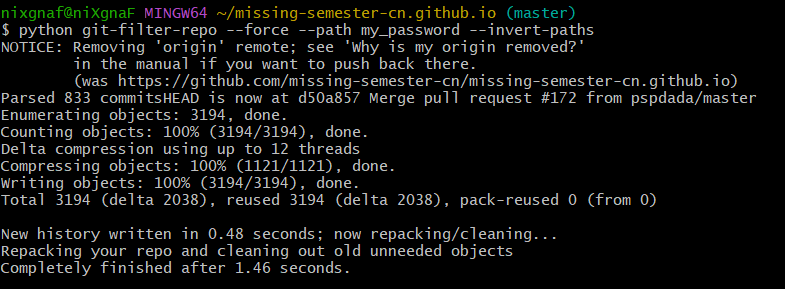
\includegraphics[width=1\linewidth]{picture/gitfilter.png}
\end{figure}

\subsection{git blame \_config.yml | grep collections}
\begin{lstlisting}
git blame _config.yml | grep collections
\end{lstlisting}

\noindent git blame \_config.yml: 显示 \_config.yml 文件的每一行的最后修改记录,包括修改者、修改时间和提交哈希。每行前面都会标记出最后修改这行的提交信息。

\noindent grep collections: 从输入中筛选出包含“collections”字符串的行。
\begin{figure}[h]
    \centering
    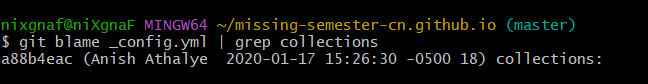
\includegraphics[width=1\linewidth]{picture/gitblame.png}
\end{figure}

\newpage
\subsection{git diff}
\begin{lstlisting}
git diff
\end{lstlisting}

\noindent git diff:显示已写入暂存区和已经被修改但尚未写入暂存区文件的区别
\begin{figure}[h]
    \centering
    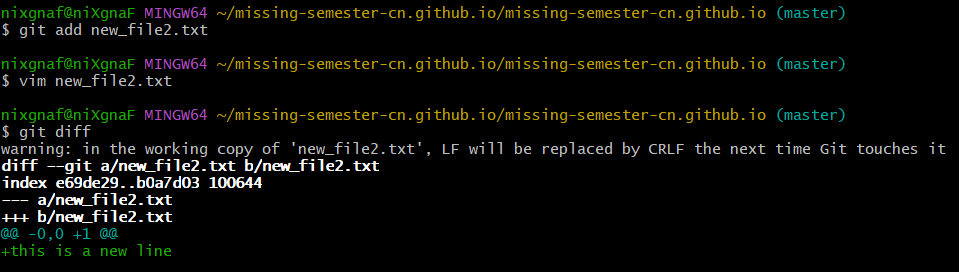
\includegraphics[width=1\linewidth]{picture/gitdiff.png}
\end{figure}

\subsection{git reset --hard HEAD~1}
\begin{lstlisting}
git reset --hard HEAD~1
\end{lstlisting}

\noindent 用于重置当前分支到上一个提交的状态,并且丢弃所有未提交的更改。

\noindent git reset:用于将当前分支的 HEAD 指针移动到指定的提交,并调整暂存区和工作目录的状态。

\noindent --hard:这个选项告诉 Git 丢弃工作目录和暂存区中的所有更改。

\noindent 指定了要重置到的目标提交。HEAD 表示当前分支的最新提交,而 HEAD~1 表示上一个提交(即当前提交的父提交)。

\begin{figure}[h]
    \centering
    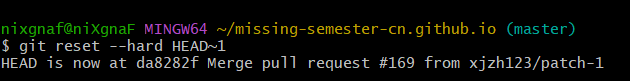
\includegraphics[width=1\linewidth]{picture/gitreset.png}
\end{figure}

\subsection{git config --list --global}
\begin{lstlisting}
git config --list --global
\end{lstlisting}

\noindent 用于列出全局配置中的所有配置项。

\noindent git config:这是 Git 的配置命令,用于查看和修改 Git 配置文件中的设置。

\noindent --list:这个选项用于列出所有当前配置项的名称和值。可以与 --global、--system 或 --local 选项一起使用,以指定查看配置的范围。
\begin{figure}[h]
    \centering
    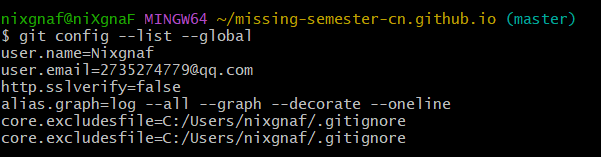
\includegraphics[width=1\linewidth]{picture/gitconfiglist.png}
\end{figure}

\newpage
\subsection{git branch dog}
\lstset{language=bash}
\begin{lstlisting}
git branch dog
\end{lstlisting}

\noindent git branch dog:创建新分支dog
\begin{figure}[h]
    \centering
    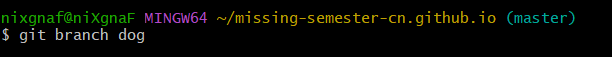
\includegraphics[width=1\linewidth]{picture/gitbranch.png}
\end{figure}

\subsection{git checkout dog}
\lstset{language=bash}
\begin{lstlisting}
git checkout dog
\end{lstlisting}

\noindent 切换到新分支dog
\begin{figure}[h]
    \centering
    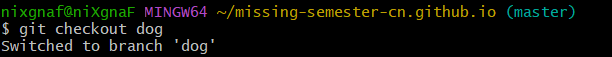
\includegraphics[width=1\linewidth]{picture/gitcheckout.png}
\end{figure}

\subsection{git branch -a -v}
\lstset{language=bash}
\begin{lstlisting}
git branch -a -v
\end{lstlisting}

\noindent 列出当前仓库的所有本地分支

\noindent -a:显示所有分支,包括本地分支和远程分支

\noindent -v:显示每个分支的最新提交摘要
\begin{figure}[h]
    \centering
    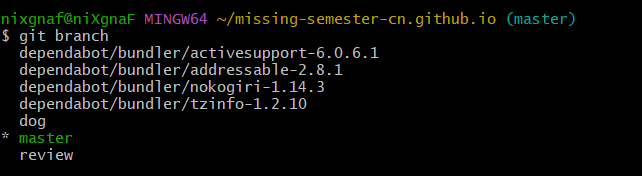
\includegraphics[width=1\linewidth]{picture/gitbrancha.png}
\end{figure}

\newpage
\subsection{git merge dog}
\lstset{language=bash}
\begin{lstlisting}
git merge dog
\end{lstlisting}

\noindent 将一个分支dog的更改合并到当前分支。
\begin{figure}[h]
    \centering
    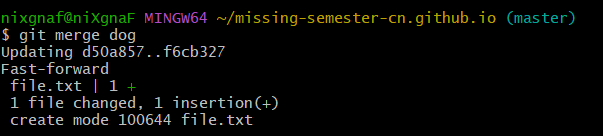
\includegraphics[width=1\linewidth]{picture/gitmerge.png}
\end{figure}

\section{实验心得}
通过本次实验,我对 Git 的工作原理有了初步理解,包括在仓库管理、提交历史查看、工作目录和暂存区操作、分支操作、配置管理等方面的基础功能,也增强了对版本控制工具在团队协作中的重要性的认识,同时进一步接触Unix系统下基于Bash语言的命令行操作。在实验报告的撰写过程中,深刻感受到Latex的精确性和专业性。


\end{document}